\chapter{nuXmv介绍}
muXmv是一种新的符号模型验证工具,主要用于有限和无限状态同步变换系统的验证与分析。nuXmv 是在经典符号模型验证工具NuSMV 的基础上创建的,不仅完全继承了NuSMV的功能,而且还从两个方面进行了拓展:1、对于有限状态系统,利用最新的SAT-based算法补充NuSMV 的基本验证技术;2、 对于无限状态系统,在NuSMV的基础上补充了两种新的数据类型,而且还提供了先进的基于SMT的形式化验证技术。除了功能上的拓展,nuXmv 还从验证性能上得到了进一步提升,nuXmv 作为一种验证工具被广泛应用于工业项目当中,例如需求分析、分布式系统模型检测、安全评估和软件模型验证。

本章节从应用角度对nuXmv的基本数据类型、模块和验证方法进行了说明,并使用具体的例子对其使用方法进行了详细的介绍。为后续的自主移动机器人移动算法建模做铺垫。

\section{基本数据类型}
在nuXmv中基本数据类型有7种,分别是布尔类型(Boolean)、枚举类型(Enumeration)、字(Word)、 整数(Integer)、 实数(Reals)、 数组(Array) 和集合(Set) 。下面对每种类型的使用做一下说明。

\paragraph{布尔类型}
类似于C++,Java等高级语言,nuXmv中的布尔类型数据只有真(TRUE)和假(FALSE)两种取值。

\paragraph{枚举类型}
同样类似于C++,Java等高级语言,枚举类型指定了该枚举的所有可能取值。举例说明:

\begin{lstlisting}
 Example 1 : {stopped, running, waiting, finished}
 Example 2 : {2, 4, -2, 0}
 Example 2 : {FAIL, 1, 3, 7, OK}
 ...
\end{lstlisting}

枚举数据类型的声明时,数据元素不能重复,数据元素的顺序没有严格要求。枚举当中元素的数据类型可以是相同的,如Example 1 中使用都是符号常量,Example 2中都是整数。也可以有混合类型的,如 Example 2 中个,既有符号常量也有整数。

\paragraph{字}
数据类型字(Word)分为无符号字(unsigned word)和有符号字(signed word),在nuXmv中分别定义语法如下:

\begin{lstlisting}
 unsigned word :unsigned word[n]
   signed word :signed word[n]
\end{lstlisting}

无符号字使用关键词unsigned word声明,有符号字使用关键词signed word。语法中n表示字的位宽(bit),例如$\left(unsigned \quad word[3]\right)$ 代表3 位(bit)的无符号字,$\left(signed \quad word[7]\right)$ 代表7位(bit)的有符号字。

\paragraph{整数}
整数有正整数和负整数。首先应该注意的是在某些模型检查引擎和算法中不允许使用整数。整型的取值范围$-2^{32}+1$ 到$2^{32}-1$。

\paragraph{实数}
实数类型的域是有理数。

\paragraph{数组}
数组使用索引的上界和下界声明。举例说明,数组$1..8$代表数组中有从1到8的8个整型元素。数组类型与集合类型不兼容,即数组元素不能是集合类型。

\paragraph{集合}
集合类型是用于标识一组值的表达式,对于集合只能使用范围常数(range constant)和联合运算符(union)。

\section{表达式}
在nuXmv中,所有的表达式都有类型的约束和操作数的类型约束,假若表达式违反了类型的约束会被系统识别为错误的表达式。下面介绍一个nuXmv 中表达式的一些性质和分类。

\subsection{隐式转换}
某些表达式操作数可以进行隐式类型转换。可以从一个类型转换成该类型的集合类型。例如,整数类型(integer)可以转换为整数集合类型(integer set)。在老版本的NuSMV中,支持整数类型(integer)隐式转换为布尔类型(boolean),但自从2.5.1版本之后不在支持整数类型(integer)隐式转换为布尔类型(boolean),同样nuXmv也不支持,只能通过必须使用显式转换运算符才能进行强制转换。


\subsection{基本表达式}
nuXmv中包含大量的基本表达式,包括最常见的逻辑运算符与、或、非等等,也包含四则运算符加、减、乘、除等等以及其他的各类操作符,下面对nuXmv中几种比较特殊的基本表达式进行介绍,其他的请参见附录[基本表达式]。

\paragraph{Case表达式}
Case表达式类似于高级语言C++,Java中的条件语言\verb|if-else if-else|。基本语法如下:

\begin{lstlisting}
    case_expr :: case case_body esac

    case_body ::
            basic_expr : basic_expr ;
          | case_body basic_expr : basic_expr ;
\end{lstlisting}

语法中\verb|case_expr|的值是\verb|case_body|中第一个左边条件为真,冒号:右边的值。下面给出一个例子,做一下简单的解释:

\begin{lstlisting}
    case
        left_expression_1 : right_expression_1 ;
        left_expression_2 : right_expression_2 ;
        ...
        left_expression_N : right_expression_N ;
    esac
\end{lstlisting}

关键词\verb|case|和\verb|esac|之间是\verb|case_body|,\verb|case_body|中所有表达式的左边条件通用表达式可以写作\verb|left_expression_[k]|,$k in {1,2,3...,N}$。对于所有的\verb|left_expression_[k]| 都必须是布尔类型。某个数值j 满足$ j in \left\{1,2,3...,N \right\}$,对于所有从1到j-1的i使得\verb|left_expression_[i]|都为FALSE,且\verb|left_expression_[j]| 为TRUE 时,case表达式的取值为\verb|left_expression_[j]|对应的右边值\verb|right_expression_[j]|。在nuXmv 中Case表达式必须有可能性的值,当所有的\verb|left_expression_[k]|都不满足时,nuXmv会抛出异常。所以会在Case表达式的最后加上一个永真条件表达式。如下:

\begin{lstlisting}
    case
        cond1 : expr1;
        cond2 : expr2;
        cond3 : expr3;
        ...
        TRUE : exprN; /*otherwise*/
    esac
\end{lstlisting}

\paragraph{Next表达式}
在nuXmv中使用Next表达式表示某个变量下一个状态时的值。其语法如下:

\begin{lstlisting}
    next_expr :: next ( basic_expr )
\end{lstlisting}

举个例子说明一下,变量V是一个状态变量,\verb|next(V)|表示变量V在下一个状态时的值。

\paragraph{取模操作}
nuXmv中使用关键字mod进行取模运算,同\verb|C/C++|程序语言中的取模的计算方法是一样的。即当a/b 是有意义的,必须使得表达式$\left(a/b\right) * b + \left(a \ mod \ b\right) = a$ 成立。下面给nuXmv 取模运算的一组实例:

\begin{lstlisting}
    7/5 = 1      7 mod 5 = 2
    -7/5 = -1   -7 mod 5 = -2
    7/-5=-1      7 mod -5 = 2
    -7/-5=1     -7 mod -5 = -2
\end{lstlisting}

\section{有限状态机}
有限状态机中可以定义变量、状态迁移关系、公平性约束等等。变量包括状态变量\verb|(state variables)|、输入变量\verb|(input variables)|和固定变量\verb|(frozen variables)|,这些变量可能随着状态的迁移,而有不同的取值。状态迁移关系表示的某个状态在不同的条件输入下,可能到达的状态。公平性约束描述状态机执行的有效路径约束。本文中所提到的约束\verb|(constraints)|是用于约束有限状态机的行为,而规格\verb|(specifications)|是用来描述有限状态机中被验证的性质。

\subsection{变量}
\subsubsection{状态变量}
状态变量使用关键词VAR进行声明,状态变量声明语法如下:

\begin{lstlisting}
var_declaration :: VAR var_list

var_list :: identifier : type_specifier ;
          | var_list identifier : type_specifier ;
\end{lstlisting}

语法中\verb|var_list|表示通过VAR关键字可以声明一组状态变量。\verb|var_list|可以是一个变量标识符\verb|identifier|,紧跟着冒号后面是改变量的类型\verb|type_specifier|。\verb|var_list identifier : type_specifier|使用递归的方式表示声明一组状态变量。下面使用一个简单的例子进行简要说明:

\begin{lstlisting}
VAR
    a : boolean;
    b : 0..10;
    c : {ready,busy};
\end{lstlisting}

例子中变量\verb|a|的类型是布尔类型。变量\verb|b|是一个限定值域范围的正数类型,其取值范围是\verb|0|到\verb|10| 之间的\verb|11|个正数。变量\verb|c|是一个枚举类型,其取值范围是枚举中两个元素\verb|ready|和\verb|busy|。


\subsubsection{输入变量}
输入变量使用关键词IVAR进行声明,常常被用于有限状态机中状态迁移关系中。输入变量的声明语法如下:

\begin{lstlisting}
ivar_declaration :: IVAR simple_var_list

simple_var_list ::
    identifier : simple_type_specifier ;
    | simple_var_list identifier : simple_type_specifier ;
\end{lstlisting}

输入变量使用只能简单的数据类型\verb|simple_type_specifier|进行,简单的数据类型包含基础的布尔类型、整数类型、实数类型等等。\verb|identifier|表示输入变量的标识符。语法中\verb|simple_var_list| 表示同状态变量声明一样,输入变量声明时也可以声明一组。

在\verb|nuXmv|中,输入变量比状态变量在使用上受到更多的限制,输入变量不能是一个模块实例。在模块和规格中同样也受到很大限制。下面给出一组具体的例子进行说明:

\begin{lstlisting}
  IVAR
    i : boolean;
  ASSIGN
    init(i) := TRUE;
    next(i) := FALSE;
\end{lstlisting}

所有的输入变量赋值都是不允许的,例子中使用关键词\verb|IVAR|声明了一个布尔类型的输入变量\verb|i|,后续使用赋值关键词\verb|ASSIGN|,定义输入变量\verb|i|的初始化值为\verb|TRUE|。 这在代码执行时,\verb|nuXmv|会返回不合法的初始化值的错误提示。

\begin{lstlisting}
  IVAR i : boolean;
   VAR s : boolean;
  INIT i = s
\end{lstlisting}

同样在INIT约束中,包含输入变量i是不合法的。

\begin{lstlisting}
    IVAR i : boolean;
     VAR s : boolean;
    TRANS i -> s;             /* 合法 */
    TRANS next(i -> s);       /* 不合法 */
\end{lstlisting}

下一个时刻状态表达式\verb|next|中,不能包含输入型变量\verb|i|。而输入变量在\verb|TRANS| 约束中,可以包含输入变量。

\begin{lstlisting}
    IVAR
       i : boolean;
    VAR
       s : boolean;
    SPEC       AF (i -> s);     /* 不合法 */
    LTLSPEC    F (X i -> s);    /* 合法 */
    INVARSPEC  (i -> s);        /* 合法 */
\end{lstlisting}

在一些规格说明语句中不能包含输入变量,这些规格说明是\verb|CTLSPEC|,\verb|SPEC|,\verb|COMPUTE|和\verb|PSLSPEC|。而对于\verb|LTLSPEC|,\verb|INVARSPEC|中包含输入变量是合法的。

\subsubsection{固定变量}
固定变量的值在状态机状态迁移过程中保持不变。固定变量的声明语法如下:

\begin{lstlisting}
    frozenvar_declaration ::
            FROZENVAR simple_var_list

    simple_var_list ::
            identifier : simple_type_specifier ;
            | simple_var_list identifier : simple_type_specifier ;
\end{lstlisting}

固定变量使用关键词FROZENVAR进行声明,\verb|simple_var_list|使用递归的表达式说明固定变量可以初始化一组。下面给出一个简单例子说明固定变量的使用场景:

\begin{lstlisting}
    FROZENVAR
         a : boolean;
         b : boolean;
         c : boolean;

    VAR  d : boolean;

    FROZENVAR e : boolean;

    ASSIGN
        init(a) := d;    /* 合法 */
        next(b) := d;    /* 不合法 */
        c := d;          /* 不合法 */
        e := a;          /* 不合法 */
\end{lstlisting}

在例子中,声明了三个固定变量a、b、c,后面定义一个状态变量d,紧跟着又定义了一个固定变量e。可以使用init对固定变量进行初始化,但不能使用next定义固定变量的下一个状态时刻的值。固定变量在初始化之后也不能使用赋值语句进行赋值操作。

\subsection{常用约束}
nuXmv中有很多种约束,这些约束可以定义模块中变量赋值、状态迁移关系、状态有效路径约束等等。比较常用的约束有INIT、ASSIGN、FAINESS等等,下面我们对常用约束做一些简单的介绍。

\subsubsection{INIT约束}
INIT约束用于定义变量的初始值,其具体语法如下:

\begin{lstlisting}
init_constrain :: INIT simple_expr [;]
\end{lstlisting}

在INIT约束中不能包含下一个状态值next的操作,表达式\verb|simple_expr|必须是布尔类型。nuXmv支持同时声明多个初始化约束。

\subsubsection{ASSIGN约束}
ASSIGN约束在nuXmv中很常见,用于给变量定义初始值,或者状态迁移时定义变量当前值和下一个状态时的值之间的等价关系。ASSIGN 约束的语法如下:

\begin{lstlisting}
assign_constraint ::
    ASSIGN assign_list

assign_list ::
    assign ;
    | assign_list assign ;

assign ::
    complex_identifier := simple_expr
    | init ( complex_identifier ) := simple_expr
    | next ( complex_identifier ) := next_expr
\end{lstlisting}

语法中\verb|assign_list|使用的是递归的表达方式,说明一个关键词ASSIGN可以定义多个ASSIGN 约束表达式。assign 中不仅支持简单的表达式\verb|simple_expr|,定义基本的等价关系,也可以使用init 关键词初始化变量值,同时也可以使用next 表达式,表示某些变量当前状态时的值和下一个状态时的值之间的等价关系。

\subsubsection{FAIRNESS约束}
在异步模型的验证过程中,常常会有一种情况是几个模型实例,它们执行的时间片是随机分配的,可能会出现一种情况就是某些模型实例的所分得时间片较少或者几乎没有。在某些应用场景中,这是不符合模型本质特性的。为了几个实例模型能够公平的获取执行时间片,nuXmv中使用关键字FAIRNESS对模块进行公平性的定义。公平性的定义很简单,只需要在模块中加上一段代码,如下:

\begin{lstlisting}
FAIRNESS
   running
\end{lstlisting}

具体的公平性的使用,将在nuXmv的模块定义中进行详细说明。



\subsection{模块的声明}
nuXmv中的模块类似于\verb|C++|,\verb|Java|等面向对象思想。在nuXmv中使用模块化的建模方式,使得代码简洁、易于阅读。模块化建模的可移植性更强,减少不必要的重复代码。nuXmv 中模块的声明语法如下:

\begin{lstlisting}
module :: MODULE identifier [( module_parameters )] [module_body]

module_parameters ::
        | module_parameters , identifier

module_body ::
          module_element
        | module_body module_element

module_element ::
          var_declaration
        | ivar_declaration
        | frozenvar_declaration
        | define_declaration
        | constants_declaration
        | assign_constraint
        | trans_constraint
        | init_constraint
        | invar_constraint
        | fairness_constraint
        | ctl_specification
        | invar_specification
        | ltl_specification
        | pslspec_specification
        | compute_specification
        | isa_declaration
        | pred_declaration
        | mirror_declaration
\end{lstlisting}

使用关键词\verb|MODULE|声明一个模块,\verb|MODULE|后面的标识符\verb|identifier|是模块的名称。模块包含两个主要的部分模块的传入参数\verb|module_parameters|和模块的主体部分\verb|module_body|。 模块的传入参数可以是一个或者多个,在给模块定义参数时,直接写参数的名称。模块的主体部分种可以定义很多种声明、约束和规格。声明包括状态变量声明\verb|var_declaration|、 输入变量声明\verb|ivar_declaration| 和固定变量声明\verb|frozenvar_declaration|等等。约束包括分配约束\verb|assign_constraint|、 初始化\verb|init_constraint|约束和公平性约束\verb|fairness_constraint|。 规格中包括线性时态规格\verb|ltl_specification|,这也是后续验证过程中使用的验证性质描述方式。nuXmv 支持同步系统和异步系统的建模,在同步系统和异步系统建模时,模块的定义是相同的,只是在一些性质的描述方面不同,下面使用二进制计数器(Binary Counter)和互斥系统(Mutual Exclusion)两个nuXmv建模的例子,分别介绍一下同步系统和异步系统的详细过程。

\paragraph{同步系统-二进制计数器}
下面程序描述一个二进制计数器,其中计数器模块\verb|counter_cell|是一个可重用的模型。在主模块main 中实例化了三个二进制计数器。

\begin{lstlisting}
MODULE counter_cell(carry_in)
    VAR
        value : boolean;
    ASSIGN
        init(value) := FALSE;
        next(value) := value xor carry_in;
    DEFINE
        carry_out := value & carry_in;

MODULE main
    VAR
        bit0 : counter_cell(TRUE);
        bit1 : counter_cell(bit0.carry_out);
        bit2 : counter_cell(bit1.carry_out);
\end{lstlisting}

程序中的主模块\verb|main|中,重复三次实例化计数器模块,分别用符号\verb|bit0|、\verb|bit1|、\verb|bit2|表示。计数器模块\verb|counter_cell| 有一个传入参数\verb|carry_in|。 在实例\verb|bit0|中,传入参数为\verb|TRUE|。在实例\verb|bit1| 中,传入参数为是实例\verb|bit0|的输出参数\verb|carry_out|。同样的,实例\verb|bit2| 的输入参数是\verb|bit1| 的输出参数\verb|carry_out|。 在计数器模块\verb|counter_cell| 中,使用关键词\verb|VAR|声明了一个布尔类型的状态变量\verb|value|。使用\verb|ASSIGN| 约束初始化了状态变量\verb|value|的值为\verb|FASLE|,和下一个状态时\verb|value|的值,下一个状态时\verb|value| 的值等于当前\verb|value| 和输入参数\verb|carry_in| 异或值\verb|value xor carry_in|。 输出变量\verb|carray_out|的值是当前状态下\verb|value|和输入变量\verb|carry_in|的与值。

\paragraph{异步系统-互斥系统}
下面模型中描述的是一个互斥系统,这是一个异步系统建模的例子。在主模块main中声明公共的布尔类型状态变量\verb|semaphore| 和两个两个模块\verb|user|的实例对象\verb|proc1|和\verb|proc2|。 并将状态变量\verb|semaphore| 作为传入参数传入\verb|proc1| 和\verb|proc2| 两个实例对象中。实例对象\verb|proc1| 和\verb|proc2|在声明时使用了关键词\verb|process|,表示\verb|proc1| 和\verb|proc2|是两个独立的异步进程。状态变量\verb|semaphore|的初始值为\verb|FALSE|。

\begin{lstlisting}
MODULE main
    VAR
        semaphore     : boolean;
        proc1         : process user(semaphore);
        proc2         : process user(semaphore);
    ASSIGN
        init(semaphore) := FALSE;

MODULE user(semaphore)
    VAR
        state : {idle, entering, critical, exiting};
    ASSIGN
        init(state) := idle;
        next(state) :=
            case
                state = idle                  : {idle, entering};
                state = entering & !semaphore : critical;
                state = critical              : {critical, exiting};
                state = exiting               : idle;
                TRUE : state;
            esac;
        next(semaphore) :=
            case
                state = entering : TRUE;
                state = exiting  : FALSE;
                TRUE             : semaphore;
            esac;
    FAIRNESS
        running
\end{lstlisting}

用户模块\verb|user|的定义中,有传入参数\verb|semaphore|。用户模块主体内部声明了状态变量\verb|state|,\verb|state|的取值有四种分别是\verb|idle|、\verb|entering|、\verb|critical| 和\verb|exiting|。状态变量\verb|state| 的初始值为\verb|idle|,下一个状态时\verb|state|的值分几种情况:当状态变量\verb|state| 是\verb|idle|时,下一个状态时变量\verb|state|取值为\verb|idle| 或者\verb|entering|,并且是随机分配的;当状态变量\verb|state|是\verb|entering|,并且传入参数\verb|semaphore| 是为\verb|FALSE|时,下一个状态时变量\verb|state|取值为\verb|critical|;当状态变量\verb|state|是\verb|critical|时,下一个状态时变量\verb|state|取值为\verb|critical| 或者\verb|exiting|,也是随机分配的;当状态变量\verb|state|是\verb|exiting| 时,下一个状态时变量\verb|state|取值为\verb|idle|;最后的\verb|TRUE :state| 条件语句,表示在不满足上述几种情况时,一个状态时变量\verb|state|取值为当前状态时\verb|state|的值。传入参数\verb|semaphore|的下一个状态时的值也使用\verb|next(semaphore)|表示:当变量\verb|state| 为\verb|entering|时,下一个状态时\verb|semaphore|的值为\verb|TRUE|;当变量\verb|state| 为\verb|exiting| 时,下一个状态时\verb|semaphore|的值为\verb|FALSE|;\verb|TRUE:semaphore|表示不满足上述两种情况时,下一个状态时\verb|semaphore|的值等于当前的\verb|semaphore| 的值。最后,在用户模块\verb|user|中使用关键词\verb|FAIRNESS| 声明了公平性,表示在异步模型中,用户模块\verb|user| 的所有实例化进程是公平的执行。

\section{交互式会话验证}
交互式会话验证是指\verb|nuXmv|模型验证的一种模式,在交互式会话验证过程中,系统的每一步操作都会停止,显示可能出现的状态值,用户可以根据自己的判断选择其中一个,\verb|nuXmv|根据用户输入完成下一步验证。当用户想验证模型中某些特殊性质时,交互式会话验证十分有用。下面使用一个例子,简单介绍一下交互式会话验证的过程。

\begin{lstlisting}
MODULE main
    VAR
       request : boolean;
         state : {ready,busy};
    ASSIGN
    	init(state) := ready;
    	next(state) :=
            case
                 state = ready & request : busy;
                 TRUE                    : {ready,busy};
            esac;
\end{lstlisting}


上面模型中主模块声明了两个状态变量\verb|request|和\verb|state|,其中变量\verb|state| 的初始值为\verb|ready|,而布尔类型变量\verb|request|的初始值并未定义,表示变量\verb|request| 的值为\verb|TRUE|或者\verb|FALSE| 中的任意一个。变量\verb|state| 在下一个状态时的值有两种情况:当\verb|state|为\verb|ready|,并且\verb|request|为\verb|TRUE|时,下一个状态时\verb|state|的值为\verb|ready|;其他情况下,下一个状态时\verb|state|的值为\verb|ready|和\verb|busy|中的任意一个。

下面是上述例子在交互式会话验证时,执行的过程:

\begin{lstlisting}
system prompt>nuXmv -int demo.smv
nuXmv > go
nuXmv > pick_state -r
nuXmv > print_current_state -v
Current state is 1.1
request = FALSE
state = ready
nuXmv > simulate -r -k 3
        Simulation Starting From State 1.1 
nuXmv > show_traces -t
There is 1 trace currently available.
nuXmv > show_traces -v
        Trace number: 1   
Trace Description: Simulation Trace
Trace Type: Simulation
  -> State: 1.1 <-
    request = FALSE
    state = ready
  -> State: 1.2 <-
    request = TRUE
    state = ready
  -> State: 1.3 <-
    request = TRUE
    state = busy
  -> State: 1.4 <-
    request = FALSE
    state = ready
nuXmv >
\end{lstlisting}

指令\verb|nuXmv -int demo.smv|中的\verb|-in|t表示\verb|nuXmv|的验证模式为交互式会话验证,\verb|demo.smv|是\verb|nuXmv| 的代码文件,内容是模型的构建代码。指令\verb|go|表示交互式会话验证开始执行。指令\verb|pick_state -r| 表示选中初始状态为验证的起始状态。指令\verb|simulate -r -k 3|表示从选择的起始状态的下一步状态开始,构建三步的状态路径。指令\verb|show_traces -v| 查看状态路径,可以在示例操作的最后看见包括初始状态在内的四个状态,每个状态都描述着变量\verb|request|和\verb|state|在当前状态下的值。根据这些状态值可以准确分析模型的状态路径。

\section{线性时态逻辑规格介绍}
通过上面的介绍,了解了\verb|nuXmv|的建模方式和适用范围。在实际适用过程中,使用\verb|nuXmv| 的建模,并验证该模型是否满足某些性质。那么此时就需要使用规格来描述这些需要验证的性质。\verb|nuXmv| 支持的规格有很多比如计算树逻辑\verb|(CTL,Computation Tree Logic)|规格、线性时态逻辑\verb|(LTL,Linear Temporal Logic)|规格、 属性说明语言\verb|PSL(Property Specification Language)| 规格等等。由于本文中使用的是线性时态逻辑规格描述机描述永恒探索算法的性质,所以此处只介绍线性时态逻辑规格。

\subsection{线性时态逻辑规格语法}

nuXmv在模块定义中使用关键词\verb|LTLSPEC|定义线性时态逻辑规格,线性时态逻辑规格的语法如下:

\begin{lstlisting}
ltl_specification ::
     LTLSPEC ltl_expr [;]

ltl_expr ::
    next_expr                    /* a next boolean expression */
    | ( ltl_expr )
    | ! ltl_expr                 /* logical not */
    | ltl_expr & ltl_expr        /* logical and */
    | ltl_expr | ltl_expr        /* logical or */
    | ltl_expr xor ltl_expr      /* logical exclusive or */
    | ltl_expr xnor ltl_expr     /* logical NOT exclusive or */
    | ltl_expr -> ltl_expr       /* logical implies */
    | ltl_expr <-> ltl_expr      /* logical equivalence */
    /*FUTURE*/
    | X ltl_expr                 /* next state */
    | G ltl_expr                 /* globally */
    | G bound ltl_expr           /* bounded globally */
    | F ltl_expr                 /* finally */
    | F bound ltl_expr           /* bounded finally */
    | ltl_expr U ltl_expr        /* until */
    | ltl_expr V ltl_expr        /* releases */
    /*PAST*/
    | Y ltl_expr                 /* previous state */
    | Z ltl_expr                 /* not previous state not */
    | H ltl_expr                 /* historically */
    | H bound ltl_expr           /* bounded historically */
    | O ltl_expr                 /* once */
    | O bound ltl_expr           /* bounded once */
    | ltl_expr S ltl_expr        /* since */
    | ltl_expr T ltl_expr        /* triggered */
bound :: [ integer_number , integer_number ]
\end{lstlisting}

线性时态逻辑规格可以包含非\verb|(!)|,与\verb|(&)|,或\verb|(|)|,异或\verb|(xor)|等逻辑运算,也可以包含线性时态逻辑中的下一个状态\verb|(X)|,某一个状态开始后续所有状态下都为真\verb|(G)|,未来某一个状态下为真\verb|(F)|等等。

下面还是使用互斥系统模型为例,简要介绍一下线性时态逻辑规格在模型中的定义:

\begin{lstlisting}
MODULE main
    VAR
        semaphore : boolean;
        proc1 : process user(semaphore);
        proc2 : process user(semaphore);
    ASSIGN
        init(semaphore) := FALSE;
    LTLSPEC G ! (proc1.state = critical & proc2.state = critical);   /* 规格1 */
    LTLSPEC G (proc1.state = entering -> F proc1.state = critical);  /* 规格2 */

MODULE user(semaphore)
    VAR
        ...
    ASSIGN
        ...
    FAIRNESS
        running
\end{lstlisting}

模型的详细内容前面已经介绍过了,这里重点解释一下主模块中新增的两条线性时态逻辑规格。规格1中描述的在未来没有一个状态时,满足进程\verb|proc1|的变量\verb|state|和进程\verb|proc1|的变量\verb|state|的值同时为\verb|critical|。规格2中描述的是当在某个状态进程\verb|proc1|变量\verb|state|的值为\verb|entering|时,在该状态之后必定有个状态满足\verb|proc1|变量\verb|state| 的值为\verb|critical|。

\section{BDD与SMT验证方法}
nuXmv支持BDD\verb|(binary decision diagram)|\cite{rr3}和SMT\verb|(Satisfiability modulo theories)|\cite{rr4}验证方式。BDD是一个有向无环图,使用二叉树的形式表示布尔逻辑函数。这种二叉分支逻辑判定的算法,可以大大减少算法的复杂度,提升判定结果集搜索效率。SMT求解方式是在SAT算法和一些优秀的求解框架的基础上发展起来的,目前SMT可满足性验证技术已经相当成熟,SMT求解器拥有较强的验证能力,并广泛应用于计算机理论、嵌入式系统、生物科学等相关领域,尤其是在大规模系统的验证中,SMT展现出十分高效的运算能力。nuXmv是一个很方便的符号模型验证工具,在集成大量优秀的形式化验证算法和求解器的同时,也对这些验证算法和求解器进行了完美的封装,提供了对应的操作和执行命令。使用者只需要按照使用手册中的说明,选择自己需要的验证方法,执行验证命令进行求解。下面分别介绍nuXmv 中的BDD和SMT的验证方法。

\paragraph{BDD验证过程}
如图\ref{fig:bddcommod}描述的是nuXmv中基于BDD验证LTL规格的命令执行流程。

\begin{figure}[!hbt]
	\centering
	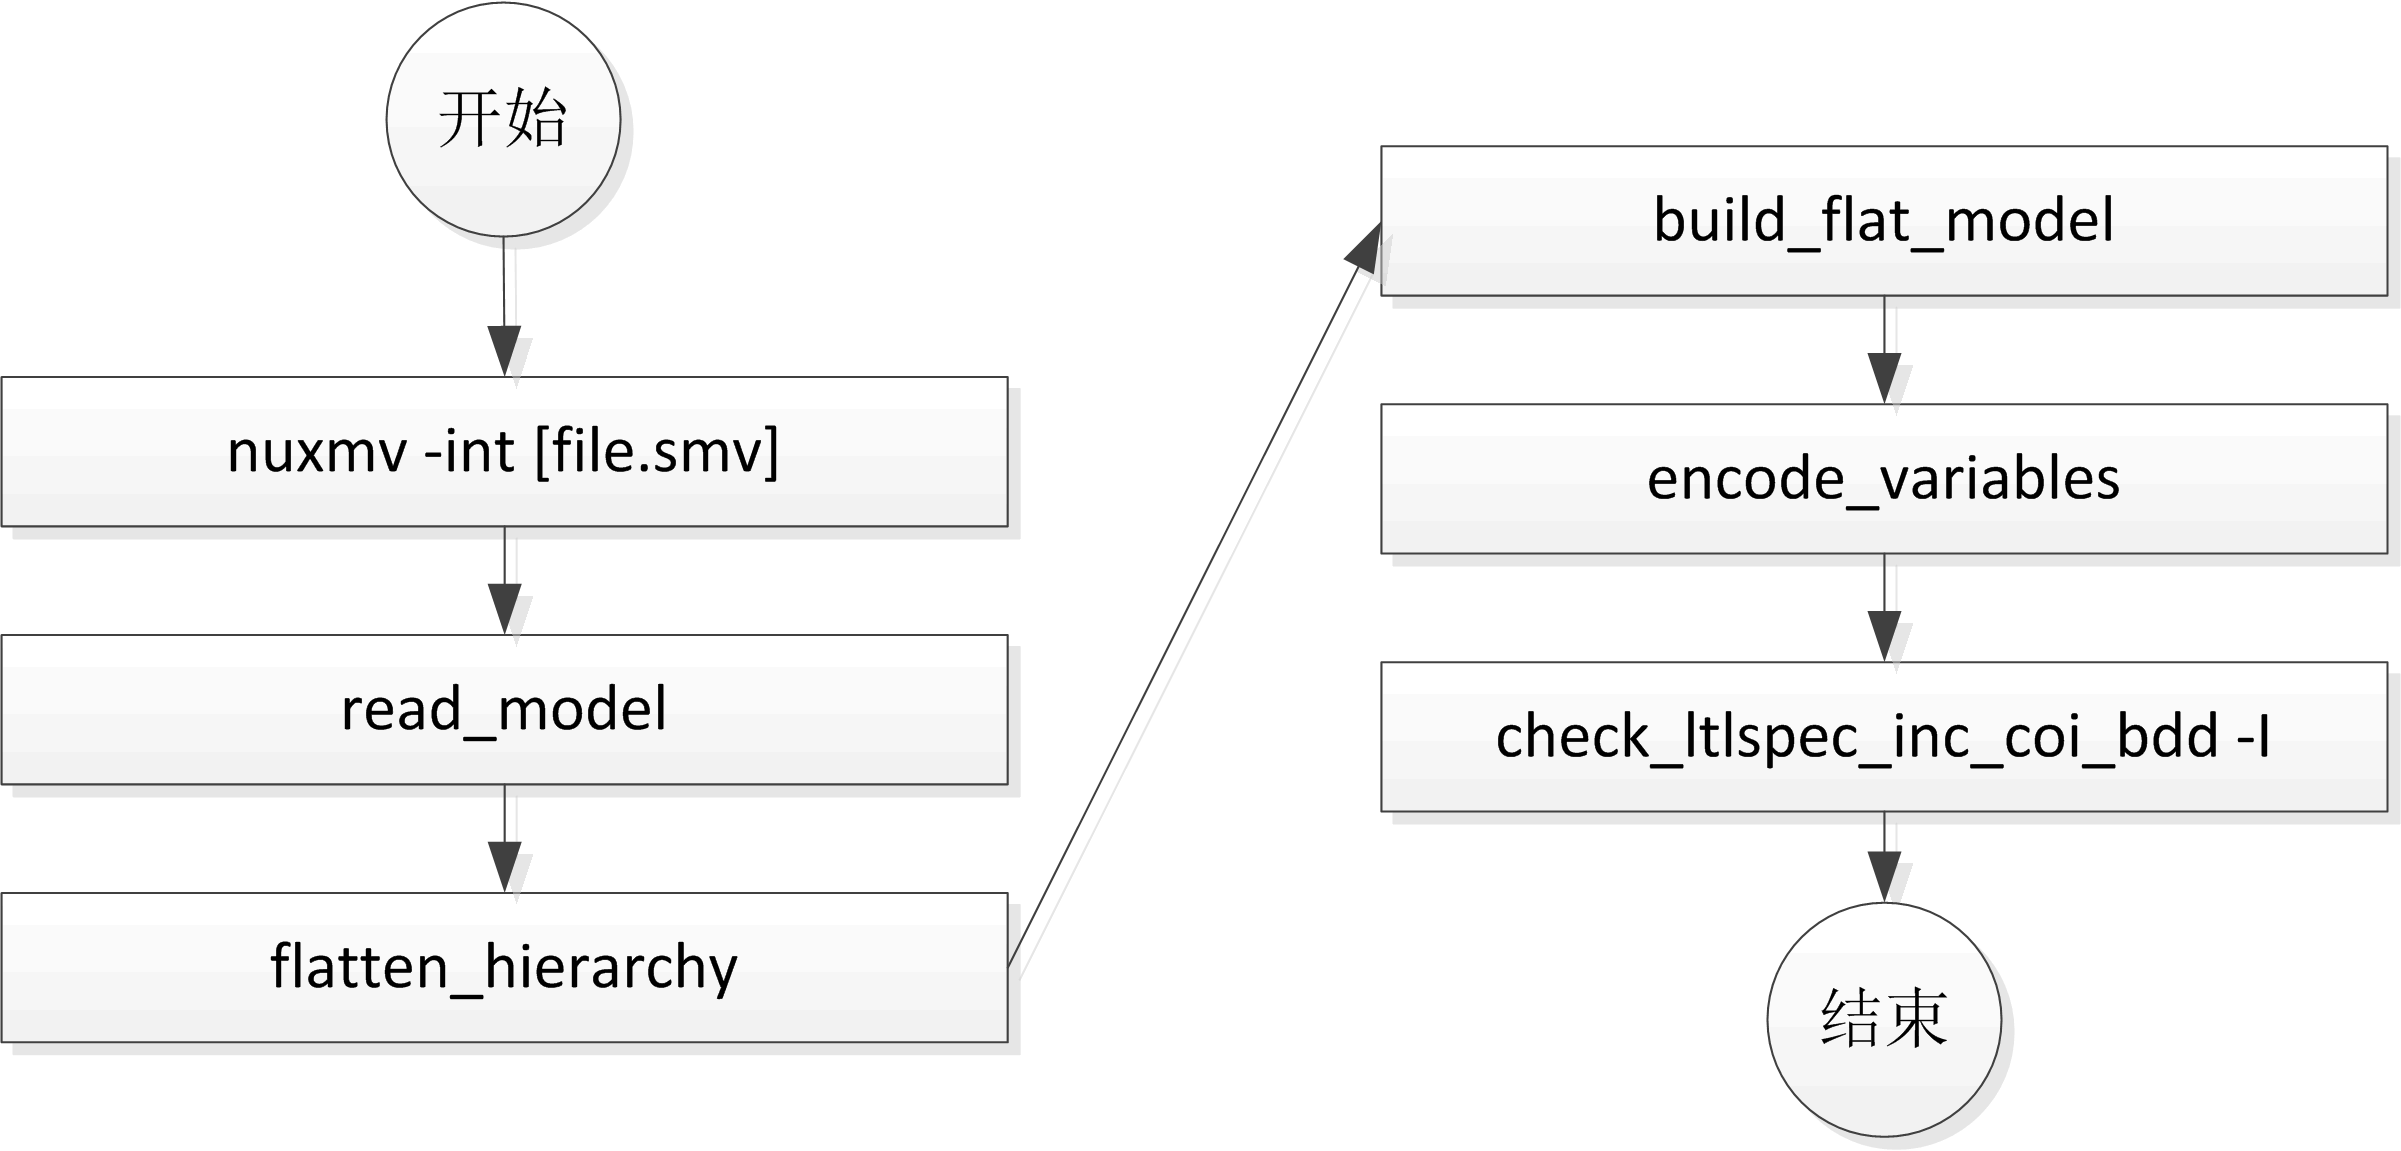
\includegraphics[width=5 in]{fig/bddcommod.png}
	\caption{基于BDD的验证方法命令流程}
	\label{fig:bddcommod}
\end{figure}

首先使用命令\verb|nuxmv -int [file.smv]|开启交互式验证模式,\verb|file.smv|是nuXmv建模文件。命令\verb|read_model|加载nuXmv的文件\verb|file.smv|到nuXmv的解析器中。命令\verb|flatten_hierarchy|通知nuXmv将建模代码中模块和过程进行偏平层次实例化。命令\verb|build_flat_model|是将偏平层次实例装配到状态机中。命令\verb|encode_variables|是构建BDD 数据结构的验证模型。命令\verb|check_ltlspec_inc_coi_bdd -I|是在BDD验证模型的基础上进行基于COI算法的LTL规格验证。

\paragraph{SMT验证过程}
如图\ref{fig:smtcommod}描述的是nuXmv中基于SMT验证LTL规格的命令执行流程。

\begin{figure}[!hbt]
	\centering
	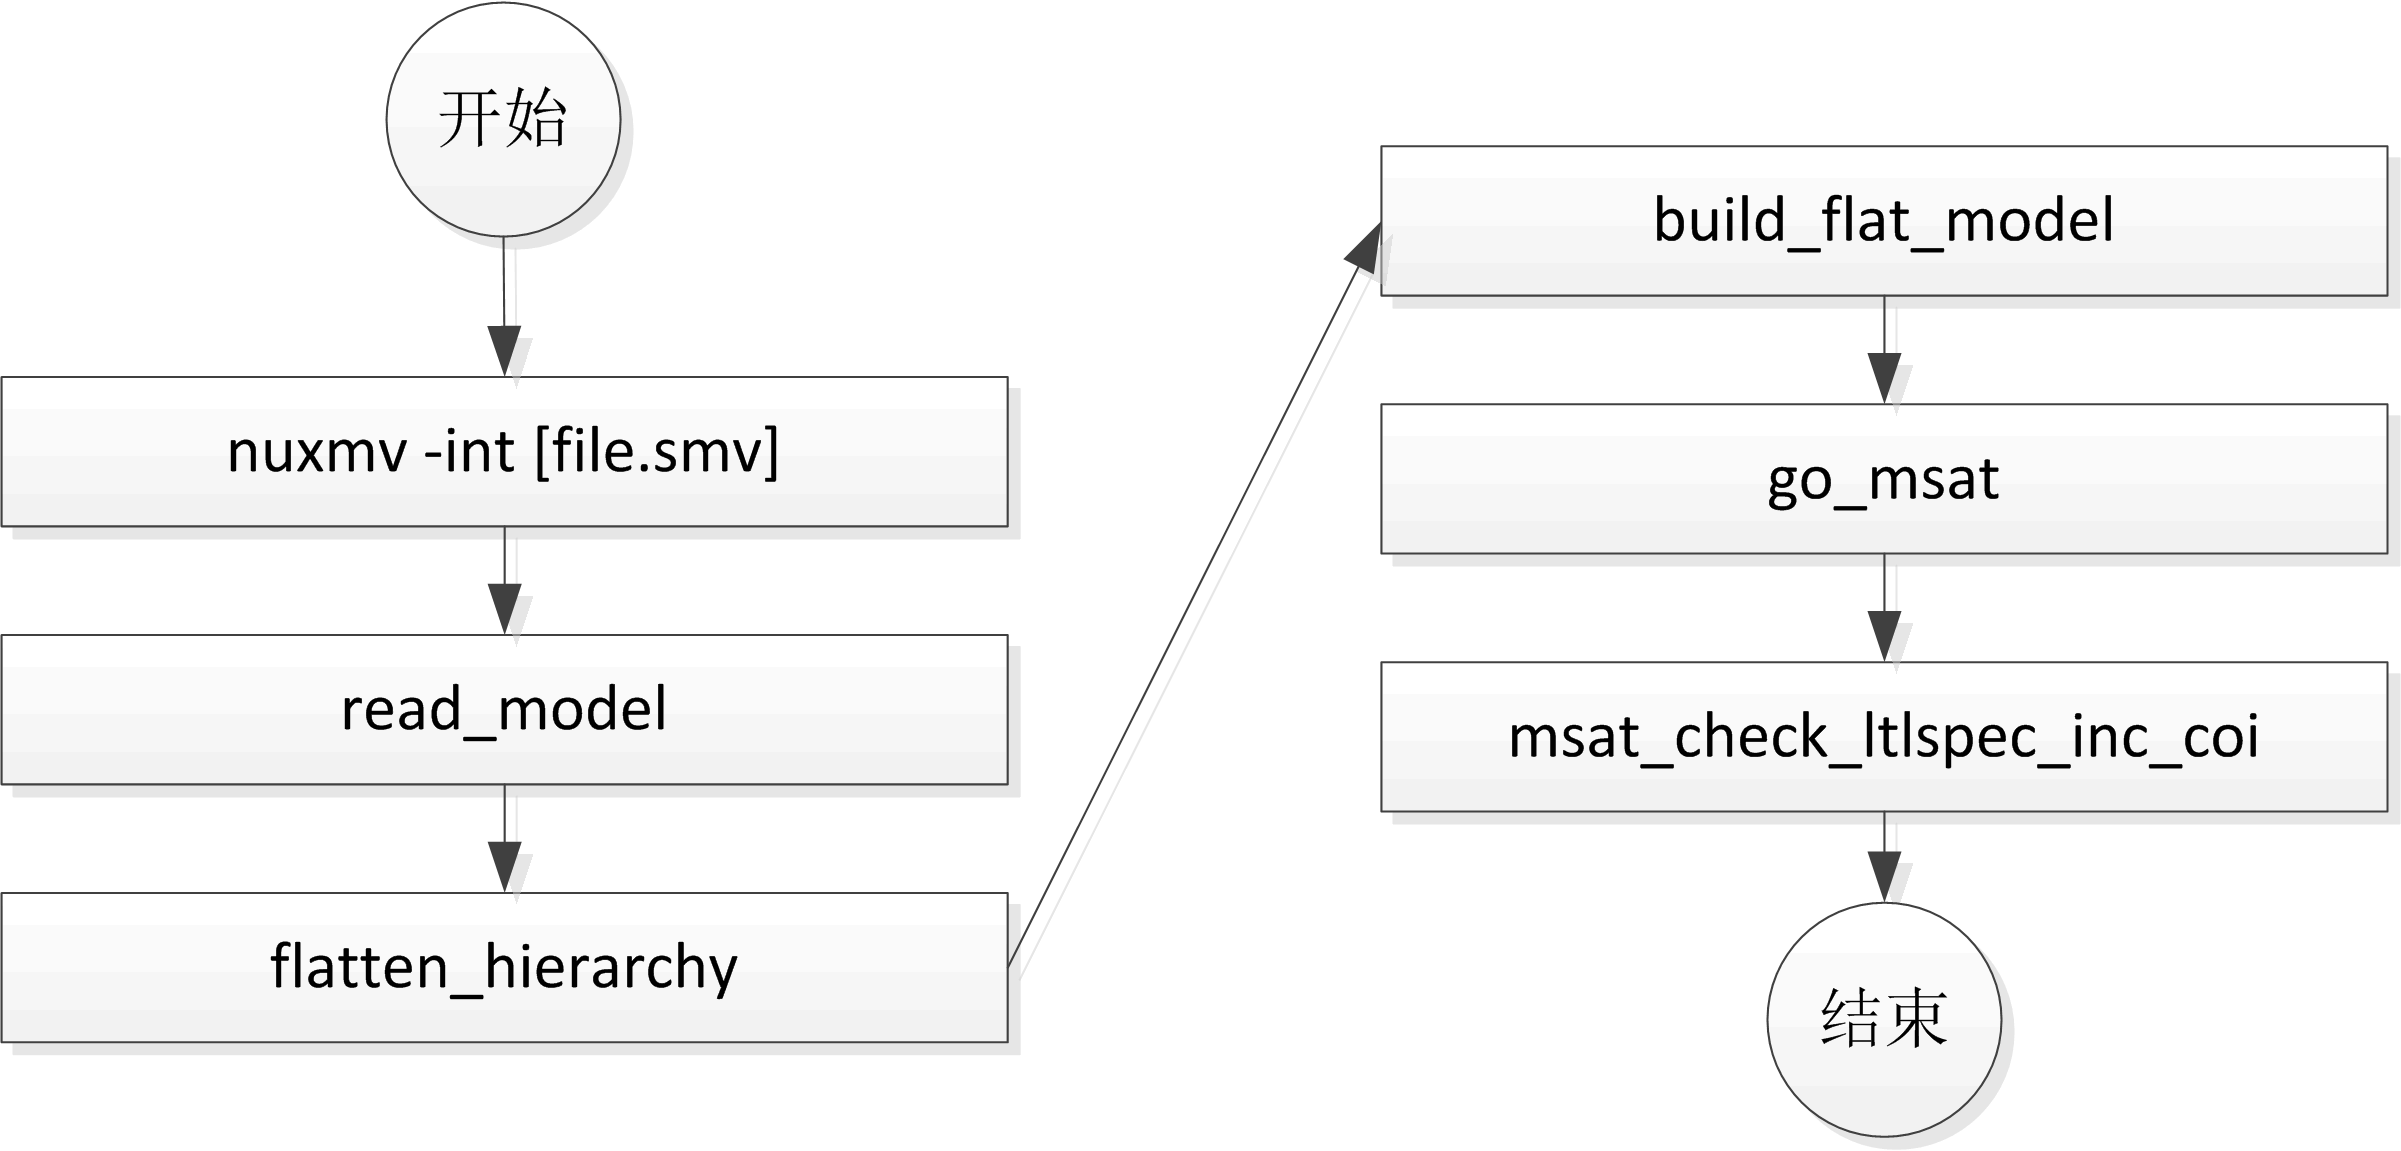
\includegraphics[width=5 in]{fig/smtcommod.png}
	\caption{基于SMT的验证方法命令流程}
	\label{fig:smtcommod}
\end{figure}

前面的执行命令与BDD验证过程中的相同,\verb|go_msat|是使用基于SMT验证方式初始化验证系统。命令\verb|msat_check_ltlspec_inc_coi|是使用基于SMT的COI算法的LTL规格验证。

\section{本章小结}
本章介绍了符号模型验证器nuXmv的基础数据类型,通过基础数据类型和模块定义可以实现有限状态机的建模。nuXmv 支持多种时序逻辑语言,本章节主要是讲解通过其中的LTL定义有限状态机中预验证性质的可满足性验证。并以异步信号系统为例,详细的介绍了模型的构建以及模块中状态迁移,重点说明LTL在模块中声明。此外,还阐述了nuXmv 支持的各种LTL的验证方法,对于验证性质的正确性,BDD 方法的效率相对较高,而对于不被满足的性质,基于SMT验证方法可以更快的找到不满足的反例。
